\documentclass{article}
\usepackage{amsmath}
\usepackage{amssymb}
\usepackage[dvipsnames, table]{xcolor}
\usepackage{pgfplots}
\usepgfplotslibrary{groupplots}
\pgfplotsset{compat=newest}
\usepackage{tikz}
\usepgfplotslibrary{fillbetween}

\begin{document}

       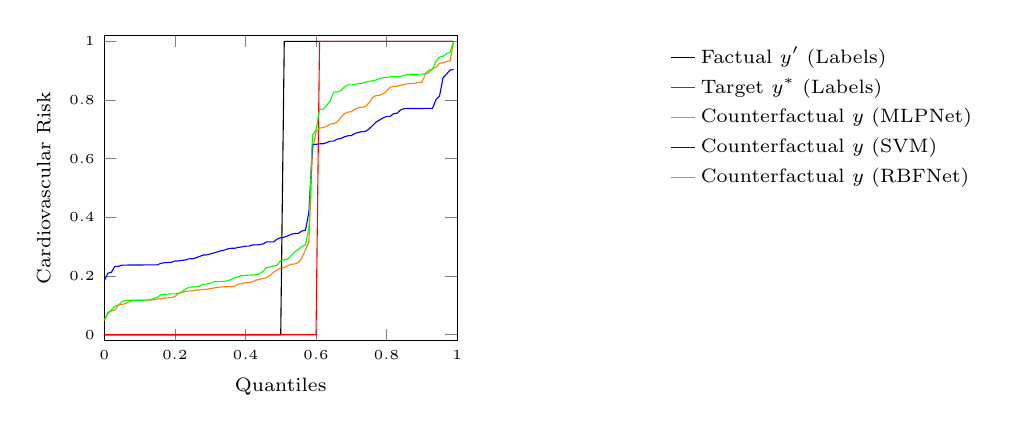
\begin{tikzpicture}
   \begin{axis}[
   title style={font=\small, yshift=-1.5ex},
   xlabel={Quantiles},
   ylabel={Cardiovascular Risk},
   xlabel style={font=\scriptsize},
   ylabel style={font=\scriptsize},
   xticklabel style={font=\tiny},
   yticklabel style={font=\tiny},
   legend style={
       draw=none,
      font=\scriptsize,
      at={(2.5, 1)}, 
      anchor=north east,
        % Custom legend line length
       legend image code/.code={
           \draw[mark repeat=2,mark phase=2]
               plot coordinates {
                   (0cm,0cm)
                   (0.3cm,0cm) % Adjust the length here
               };
       },
   },
   xmin=0, xmax=1,
   ymin=-0.02, ymax=1.02,
   grid style=dashed,
   legend cell align={left},
   width=0.5\linewidth,
   height=0.45\linewidth,
   scaled x ticks=false,
   xticklabel style={/pgf/number format/fixed}
   ]

   % Hypothetical quantile function for the first distribution
   \addplot[
       color=black,
       ]
       coordinates {
(0.0,0.0) (0.01,0.0) (0.02,0.0) (0.03,0.0) (0.04,0.0) (0.05,0.0) (0.06,0.0) (0.07,0.0) (0.08,0.0) (0.09,0.0) (0.1,0.0) (0.11,0.0) (0.12,0.0) (0.13,0.0) (0.14,0.0) (0.15,0.0) (0.16,0.0) (0.17,0.0) (0.18,0.0) (0.19,0.0) (0.2,0.0) (0.21,0.0) (0.22,0.0) (0.23,0.0) (0.24,0.0) (0.25,0.0) (0.26,0.0) (0.27,0.0) (0.28,0.0) (0.29,0.0) (0.3,0.0) (0.31,0.0) (0.32,0.0) (0.33,0.0) (0.34,0.0) (0.35,0.0) (0.36,0.0) (0.37,0.0) (0.38,0.0) (0.39,0.0) (0.4,0.0) (0.41,0.0) (0.42,0.0) (0.43,0.0) (0.44,0.0) (0.45,0.0) (0.46,0.0) (0.47,0.0) (0.48,0.0) (0.49,0.0) (0.5,0.0) (0.51,1.0) (0.52,1.0) (0.53,1.0) (0.54,1.0) (0.55,1.0) (0.56,1.0) (0.57,1.0) (0.58,1.0) (0.59,1.0) (0.6,1.0) (0.61,1.0) (0.62,1.0) (0.63,1.0) (0.64,1.0) (0.65,1.0) (0.66,1.0) (0.67,1.0) (0.68,1.0) (0.69,1.0) (0.7,1.0) (0.71,1.0) (0.72,1.0) (0.73,1.0) (0.74,1.0) (0.75,1.0) (0.76,1.0) (0.77,1.0) (0.78,1.0) (0.79,1.0) (0.8,1.0) (0.81,1.0) (0.82,1.0) (0.83,1.0) (0.84,1.0) (0.85,1.0) (0.86,1.0) (0.87,1.0) (0.88,1.0) (0.89,1.0) (0.9,1.0) (0.91,1.0) (0.92,1.0) (0.93,1.0) (0.94,1.0) (0.95,1.0) (0.96,1.0) (0.97,1.0) (0.98,1.0) (0.99,1.0)



       };
       \addlegendentry{Factual $y'$ (Labels)}

   % Hypothetical quantile function for the second distribution
   \addplot[
       color=red,
       ]
       coordinates {
(0.0,0.0) (0.01,0.0) (0.02,0.0) (0.03,0.0) (0.04,0.0) (0.05,0.0) (0.06,0.0) (0.07,0.0) (0.08,0.0) (0.09,0.0) (0.1,0.0) (0.11,0.0) (0.12,0.0) (0.13,0.0) (0.14,0.0) (0.15,0.0) (0.16,0.0) (0.17,0.0) (0.18,0.0) (0.19,0.0) (0.2,0.0) (0.21,0.0) (0.22,0.0) (0.23,0.0) (0.24,0.0) (0.25,0.0) (0.26,0.0) (0.27,0.0) (0.28,0.0) (0.29,0.0) (0.3,0.0) (0.31,0.0) (0.32,0.0) (0.33,0.0) (0.34,0.0) (0.35,0.0) (0.36,0.0) (0.37,0.0) (0.38,0.0) (0.39,0.0) (0.4,0.0) (0.41,0.0) (0.42,0.0) (0.43,0.0) (0.44,0.0) (0.45,0.0) (0.46,0.0) (0.47,0.0) (0.48,0.0) (0.49,0.0) (0.5,0.0) (0.51,0.0) (0.52,0.0) (0.53,0.0) (0.54,0.0) (0.55,0.0) (0.56,0.0) (0.57,0.0) (0.58,0.0) (0.59,0.0) (0.6,0.0) (0.61,1.0) (0.62,1.0) (0.63,1.0) (0.64,1.0) (0.65,1.0) (0.66,1.0) (0.67,1.0) (0.68,1.0) (0.69,1.0) (0.7,1.0) (0.71,1.0) (0.72,1.0) (0.73,1.0) (0.74,1.0) (0.75,1.0) (0.76,1.0) (0.77,1.0) (0.78,1.0) (0.79,1.0) (0.8,1.0) (0.81,1.0) (0.82,1.0) (0.83,1.0) (0.84,1.0) (0.85,1.0) (0.86,1.0) (0.87,1.0) (0.88,1.0) (0.89,1.0) (0.9,1.0) (0.91,1.0) (0.92,1.0) (0.93,1.0) (0.94,1.0) (0.95,1.0) (0.96,1.0) (0.97,1.0) (0.98,1.0) (0.99,1.0)
       };
       \addlegendentry{Target $y^*$ (Labels)}

   \addplot[
       color=orange,
   ]
   coordinates {
    (0.0,0.048134) (0.01,0.07646) (0.02,0.080828) (0.03,0.084128) (0.04,0.101229) (0.05,0.103247) (0.06,0.106219) (0.07,0.111953) (0.08,0.116654) (0.09,0.117398) (0.1,0.117465) (0.11,0.117783) (0.12,0.117958) (0.13,0.118062) (0.14,0.119295) (0.15,0.121822) (0.16,0.12226) (0.17,0.125054) (0.18,0.125662) (0.19,0.127109) (0.2,0.129525) (0.21,0.141494) (0.22,0.144456) (0.23,0.147517) (0.24,0.14868) (0.25,0.149598) (0.26,0.152413) (0.27,0.152612) (0.28,0.154169) (0.29,0.154931) (0.3,0.157383) (0.31,0.15901) (0.32,0.161521) (0.33,0.162547) (0.34,0.163527) (0.35,0.163714) (0.36,0.163815) (0.37,0.16453) (0.38,0.173303) (0.39,0.173625) (0.4,0.177459) (0.41,0.177924) (0.42,0.18045) (0.43,0.185905) (0.44,0.188964) (0.45,0.191822) (0.46,0.194386) (0.47,0.202976) (0.48,0.213145) (0.49,0.220688) (0.5,0.227564) (0.51,0.228996) (0.52,0.235626) (0.53,0.240168) (0.54,0.241244) (0.55,0.246224) (0.56,0.261551) (0.57,0.289598) (0.58,0.317896) (0.59,0.627002) (0.6,0.69088) (0.61,0.704609) (0.62,0.705802) (0.63,0.710005) (0.64,0.718468) (0.65,0.719291) (0.66,0.725229) (0.67,0.739858) (0.68,0.75347) (0.69,0.758725) (0.7,0.760235) (0.71,0.768568) (0.72,0.773452) (0.73,0.775532) (0.74,0.777412) (0.75,0.790069) (0.76,0.808646) (0.77,0.815419) (0.78,0.816155) (0.79,0.821147) (0.8,0.830516) (0.81,0.843665) (0.82,0.846648) (0.83,0.846789) (0.84,0.850471) (0.85,0.853076) (0.86,0.855702) (0.87,0.856911) (0.88,0.856972) (0.89,0.859193) (0.9,0.860678) (0.91,0.887495) (0.92,0.893584) (0.93,0.906902) (0.94,0.911537) (0.95,0.924957) (0.96,0.926847) (0.97,0.931793) (0.98,0.933517) (0.99,0.999948)
   };
   \addlegendentry{Counterfactual $y$ (MLPNet)}

   \addplot[
       color=blue,
   ]
   coordinates {
(0.0,0.184034) (0.01,0.209718) (0.02,0.21292) (0.03,0.232998) (0.04,0.233065) (0.05,0.237304) (0.06,0.237369) (0.07,0.23754) (0.08,0.237665) (0.09,0.237676) (0.1,0.237704) (0.11,0.237837) (0.12,0.237882) (0.13,0.237918) (0.14,0.237947) (0.15,0.237948) (0.16,0.243224) (0.17,0.245389) (0.18,0.246176) (0.19,0.247066) (0.2,0.251085) (0.21,0.251563) (0.22,0.253309) (0.23,0.254699) (0.24,0.258683) (0.25,0.25891) (0.26,0.26203) (0.27,0.26674) (0.28,0.271724) (0.29,0.27196) (0.3,0.275465) (0.31,0.278265) (0.32,0.28223) (0.33,0.286117) (0.34,0.288391) (0.35,0.292666) (0.36,0.294616) (0.37,0.29477) (0.38,0.297628) (0.39,0.299419) (0.4,0.301728) (0.41,0.30189) (0.42,0.305959) (0.43,0.306051) (0.44,0.307141) (0.45,0.309508) (0.46,0.316239) (0.47,0.316392) (0.48,0.316683) (0.49,0.326244) (0.5,0.330323) (0.51,0.332811) (0.52,0.336754) (0.53,0.342486) (0.54,0.345112) (0.55,0.345338) (0.56,0.353811) (0.57,0.355725) (0.58,0.419265) (0.59,0.648424) (0.6,0.649068) (0.61,0.650692) (0.62,0.651018) (0.63,0.654431) (0.64,0.660094) (0.65,0.660128) (0.66,0.66631) (0.67,0.669187) (0.68,0.674263) (0.69,0.678164) (0.7,0.678997) (0.71,0.685911) (0.72,0.689638) (0.73,0.691877) (0.74,0.6931) (0.75,0.701035) (0.76,0.712812) (0.77,0.724595) (0.78,0.731887) (0.79,0.738776) (0.8,0.744028) (0.81,0.744127) (0.82,0.753754) (0.83,0.754986) (0.84,0.766525) (0.85,0.770845) (0.86,0.771038) (0.87,0.77104) (0.88,0.771052) (0.89,0.771177) (0.9,0.771224) (0.91,0.77134) (0.92,0.77147) (0.93,0.771508) (0.94,0.801439) (0.95,0.813303) (0.96,0.875823) (0.97,0.888618) (0.98,0.902107) (0.99,0.903687)
   };
   \addlegendentry{Counterfactual $y$ (SVM)}

   \addplot[
       color=green,
   ]
   coordinates {
(0.0,0.05007) (0.01,0.071719) (0.02,0.083807) (0.03,0.096894) (0.04,0.100011) (0.05,0.112778) (0.06,0.117262) (0.07,0.117496) (0.08,0.117498) (0.09,0.117505) (0.1,0.11755) (0.11,0.117557) (0.12,0.118172) (0.13,0.119554) (0.14,0.123147) (0.15,0.127119) (0.16,0.136288) (0.17,0.138016) (0.18,0.138448) (0.19,0.13918) (0.2,0.139212) (0.21,0.139796) (0.22,0.146326) (0.23,0.155174) (0.24,0.162262) (0.25,0.162657) (0.26,0.164757) (0.27,0.165423) (0.28,0.172139) (0.29,0.172433) (0.3,0.174703) (0.31,0.180177) (0.32,0.180924) (0.33,0.181253) (0.34,0.182075) (0.35,0.184099) (0.36,0.188346) (0.37,0.194468) (0.38,0.19783) (0.39,0.201754) (0.4,0.202211) (0.41,0.203184) (0.42,0.20367) (0.43,0.204545) (0.44,0.207768) (0.45,0.216469) (0.46,0.228624) (0.47,0.23067) (0.48,0.234557) (0.49,0.237039) (0.5,0.252618) (0.51,0.255269) (0.52,0.258358) (0.53,0.270614) (0.54,0.282552) (0.55,0.291063) (0.56,0.300976) (0.57,0.305788) (0.58,0.364877) (0.59,0.679752) (0.6,0.696714) (0.61,0.767996) (0.62,0.769294) (0.63,0.781509) (0.64,0.796918) (0.65,0.82687) (0.66,0.827691) (0.67,0.831358) (0.68,0.844014) (0.69,0.851577) (0.7,0.851628) (0.71,0.852545) (0.72,0.856325) (0.73,0.856807) (0.74,0.861041) (0.75,0.863733) (0.76,0.865504) (0.77,0.868324) (0.78,0.872806) (0.79,0.876397) (0.8,0.87646) (0.81,0.879068) (0.82,0.880438) (0.83,0.880632) (0.84,0.880699) (0.85,0.884476) (0.86,0.887539) (0.87,0.887757) (0.88,0.887884) (0.89,0.888038) (0.9,0.888131) (0.91,0.890307) (0.92,0.901975) (0.93,0.904423) (0.94,0.932436) (0.95,0.946241) (0.96,0.949443) (0.97,0.958157) (0.98,0.962398) (0.99,1.0)
   };
   \addlegendentry{Counterfactual $y$ (RBFNet)}
   \end{axis}
   \end{tikzpicture}

\end{document}